
\section*{CHƯƠNG 2. PHÂN TÍCH HỆ THỐNG}
\setcounter{section}{2}
\setcounter{subsection}{0} %LƯU Ý MỖI LẦN THÊM CHƯƠNG MỚI CẦN THÊM CÂU NÀY ĐỂ RESET THỨ TỰ CỦA SUBSECTON VỀ 1
\setcounter{table}{0} % LƯU Ý SAU MỖI LẦN GỌI BẢNG HAY HÌNH ẢNH PHẢI THÊM CÂU NÀY ĐỂ RESET THỨ TỰ
\setcounter{figure}{0} %% LƯU Ý SAU MỖI LẦN GỌI BẢNG HAY HÌNH ẢNH PHẢI THÊM CÂU NÀY ĐỂ RESET THỨ TỰ
\addcontentsline{toc}{section}{\numberline{}CHƯƠNG 2. PHÂN TÍCH HỆ THỐNG}
Chương này sẽ trình bày chi tiết về quá trình phân tích hệ thống, dựa trên các yêu cầu đã được nêu trong Phần mở đầu và Chương 1. Quá trình này bao gồm các bước sau:\begin{adjustwidth}{1.5em}{}
  \begin{itemize}
    \item Thiết kế các thẻ CRC (Class - Responsibility - Collaboration Card) cùng các lớp dựa trên thông tin từ các sơ đồ use case chức năng của hệ thống
    \item Xây dựng sơ đồ lớp dựa trên các lớp đã được định nghĩa với thuộc tính và phương thức
    \item Sau khi đã xác định về phương thức cũng như thuộc tính các lớp cùng chức năng, bước tiếp theo sẽ thiết kế các sơ đồ tuần tự minh họa sự tương tác giữa các lớp 
          khi thực hiện chức năng cụ thể
  \end{itemize}
  \end{adjustwidth}
% \newpage
\subsection{Thẻ CRC (Class - Responsibility - Collaboration Card)}

\subsubsection{Thẻ CRC lớp account}
\subsubsection{Thẻ CRC lớp user role}

\subsubsection{Thẻ CRC lớp user status}

\subsubsection{Thẻ CRC lớp users}

\subsubsection{Thẻ CRC lớp device type}

\subsubsection{Thẻ CRC lớp device status}

\subsubsection{Thẻ CRC lớp devices}

\subsubsection{Thẻ CRC lớp device details}
\subsubsection{Thẻ CRC lớp records}

\subsubsection{Thẻ CRC lớp record diagnosis}

\subsubsection{Thẻ CRC lớp notification schedule}

\subsubsection{Thẻ CRC lớp schedule type}

\subsubsection{Thẻ CRC lớp schedule status}

\subsubsection{Thẻ CRC lớp schedules}

\subsubsection{Thẻ CRC lớp diagnosis}

\subsubsection{Thẻ CRC lớp device type}

\subsubsection{Thẻ CRC lớp consultation schedule}





\begin{xltabular}{\textwidth}{
   >{\centering\arraybackslash}X 
  }
  \caption{\bfseries \fontsize{12pt}{0pt}\selectfont Thẻ CRC lớp Người dùng}
  % \label{table_api_news}
  \\
  \begin{tabularx}{0.9\textwidth}{X}
    Mặt trước thẻ
  \end{tabularx}
  \begin{tabularx}{0.9\textwidth}{|X|X|}
    \hline
    \textbf{Tên lớp:} Người dùng (User) & \textbf{ID:} 1 \\
    \hline
    \textbf{Mô tả:} Đối tượng mô tả thông tin người dùng & \textbf{Use case liên quan:}  Đăng ký tài khoản, Quản lý tài khoản cá nhân, Quản lý phân công bác sĩ - bệnh nhân\\
    \hline
    \textbf{Trách nhiệm (Responsibility):} & \textbf{Các lớp cộng tác (Collaboration):} \\
    Thêm, sửa, xóa thông tin người dùng 

    Lấy danh sách người dùng

    Lấy thông tin người dùng qua ID, tài khoản, chức vụ
    & 
    Tài khoản
    \\
    \hline
  \end{tabularx}
  \\ 
  \begin{tabularx}{0.9\textwidth}{X}
    Mặt sau thẻ
  \end{tabularx} 
  \begin{tabularx}{0.9\textwidth}{|X|X|}
    \hline
    \textbf{Thuộc tính (Attributes):} & \\
    id(uuid) 
    
    username(String)

    birth(Timestamps)

    phone\_number(String)
    & 
    image(String) 
    
    role(Integer) 
    
    created\_at(Timestamps)

    updated\_at(Timestamps)
    \\ \hline
  \end{tabularx}
  \\     
  \begin{tabularx}{0.9\textwidth}{|X|}
    \hline
   \textbf{Mối quan hệ (Relationships)} \\
    Tổng quát hóa (Generalize):  

    Toàn thể - Bộ phận (Aggregation):
    
    Liên kết (Association): Tài khoản, Phân công bác sĩ - bệnh nhân 
    \\
    \hline
  \end{tabularx}
  \end{xltabular}

  \begin{xltabular}{\textwidth}{
    >{\centering\arraybackslash}X 
  }
  \caption{\bfseries \fontsize{12pt}{0pt}\selectfont Thẻ CRC lớp Tệp đính kèm}
  % \label{table_api_news}
  \\
  \begin{tabularx}{0.9\textwidth}{X}
    Mặt trước thẻ
  \end{tabularx}
  \begin{tabularx}{0.9\textwidth}{|X|X|}
    \hline
    \textbf{Tên lớp:} Tệp đính kèm & \textbf{ID:} 14 \\
    \hline
    \textbf{Mô tả:} Đối tượng mô tả thông tin Tệp đính kèm tin nhắn & \textbf{Use case liên quan:} Quản lý dịch vụ nhắn tin \\
    \hline
    \textbf{Trách nhiệm (Responsibility):} & \textbf{Các lớp cộng tác (Collaboration):} \\
    Mô tả thông tin Tệp đính kèm

    Lấy thông tin tệp đính kèm theo tin nhắn, cuộc hội thoại
    & 
    Tin nhắn, Cuộc hội thoại
    \\
    \hline
  \end{tabularx}
  \\ 
  \begin{tabularx}{0.9\textwidth}{X}
    Mặt sau thẻ
  \end{tabularx} 
  \begin{tabularx}{0.9\textwidth}{|X|X|}
    \hline
    \textbf{Thuộc tính (Attributes):} & \\
    id(String) 

    content\_url(String)
    
    file\_name(String)
    &
    size(Integer)

    thumbnail\_url(String)

    type(Integer)
    \\
    \hline
  \end{tabularx}
  \\     
  \begin{tabularx}{0.9\textwidth}{|X|}
    \textbf{Mối quan hệ (Relationships):} \\
    Tổng quát hóa (Generalize):  

    Toàn thể - Bộ phận (Aggregation): 
    
    Liên kết (Association): Tin nhắn, Cuộc hội thoại 
    \\
    \hline
  \end{tabularx}
  \end{xltabular}


% \newpage
\subsection{Sơ đồ lớp}
  Dựa trên các thẻ CRC đã được mô tả ở phần trên, chúng em xin phép trình bày về sơ đồ lớp của hệ thống.

  % Hình \ref*{UML} thể hiện các lớp trong hệ thống:
  % \begin{itemize}
  %   \item Lớp Account (Tài khoản): Lớp thể hiện cho cấu trúc của một account khi đăng ký sử dụng hệ thống, cung cấp các hàm và các biến để thực hiện chức năng đăng ký người dùng
  %   \item Lớp Register (Tài khoản phê duyệt): Lớp thể hiện cho cấu trúc của người dùng khi mới đăng ký, cung cấp các hàm, phương thức thao tác dữ liệu người dùng khi mới đăng ký
  %   \item Lớp User (Người dùng): Lớp thể hiện cho cấu trúc của người dùng sau khi đã đăng ký, cung cấp các hàm, phương thức liên quan đến dữ liệu người dùng sau đăng ký
  %   \item Lớp Token: Lớp thể hiện cho cấu trúc của một token, cung cấp biến, hàm để thao tác với người dùng khi thực hiện đăng ký, đăng nhập
  %   \item Lớp PatientDoctorAssignment (Phân công bác sĩ - bệnh nhân): Lớp thể hiện cho cấu trúc của một bảng phân công giữa bệnh nhân và bác sĩ, cung cấp các hàm, phương thức để lấy dữ liệu phân công bệnh nhân/bác sĩ
  %   \item Lớp Record (Bản ghi): Lớp thể hiện cho cấu trúc của một bản ghi record, cung cấp các hàm, phương thức để thực hiện liên quan đến các bản ghi dữ liệu sức khỏe của bệnh nhân
  %   \item Lớp Device (Thiết bị): Lớp thể hiện cho cấu trúc của một thiết bị, cung cấp các biến, hàm, phương thức để thực hiện liên quan đến thông tin các thiết bị sử dụng trong các ghi record
  %   \item Lớp DeviceDetail (Thông số thiết bị): Lớp thể hiện cho cấu trúc của chi tiết liên quan đến lớp thiết bị, cung cấp các hàm, phương thức để thực hiện thao tác với dữ liệu các thiết bị và các bản ghi record
  %   \item Lớp News (Tin tức): Lớp thể hiện cho cấu trúc của một tin tức, cung cấp các hàm, phương thức để lấy dữ liệu tin tức
  %   \item Lớp NewsCategories (Danh mục tin tức): Lớp thể hiện cho cấu trúc của một danh mục tin tức, cung cấp các hàm, phương thức để lấy dữ liệu từ danh mục tin tức
  %   \item Lớp Conversation (Cuộc hội thoại): Lớp thể hiện cho cấu trúc của một cuộc hội thoại, cung cấp các biến, hàm, phương thức để lấy dữ liệu liên quan đến cuộc hội thoại
  %   \item Lớp ConversationMember (Thành viên tham gia hội thoại): Lớp thể hiện cho cấu trúc của danh sách những người tham gia một cuộc hội thoại, cung cấp các hàm, phương thức để xử lý dữ liệu liên quan đến người dùng
  %   \item Lớp ConversationAttachment (Tệp đính kèm): Lớp thể hiện cho cấu trúc của danh sách những tệp được đính kém trong danh sách hội thoại, cung cấp các hàm, phương thức để xử lý các chức năng liên quan đến hội thoại
  %   \item Lớp Message (Tin nhắn): Lớp thể hiện cho cấu trúc của một message được sử dụng trong hội thoại, cung cấp các hàm, phương thức để xử lý dữ liệu trong cuộc hội thoại
  % \end{itemize}
% \newpage
\subsection{Sơ đồ tuần tự}
Để phân tích cụ thể hơn về từng luồng trong hệ thống thông qua sơ đồ use case và sơ đồ hoạt động, dưới đây là phần thiết kế
 về các sơ đồ tuần tự.

\subsubsection{Sơ đồ tuần tự đăng ký tài khoản}

Sơ đồ tuần tự mô tả chi tiết quá trình người dùng đăng ký một tài khoản mới trên hệ thống. Người dùng sẽ phải gửi yêu cầu đăng ký, hệ thống sẽ được xử lý
bởi lớp Register, nếu có lỗi phát sinh hệ thống sẽ thông báo lõi cho người dùng. Nếu việc đăng ký thành công, lớp Register sẽ gửi thông báo 
chuyển sang phê duyệt tài khoản và trả về kết quả.  


\subsubsection{Sơ đồ tuần tự đăng nhập tài khoản}
\subsubsection{Sơ đồ tuần tự lấy tất cả người dùng}

\subsubsection{Sơ đồ tuần tự lấy người dùng theo id}

\subsubsection{Sơ đồ tuần tự cập nhật người dùng theo id}

\subsubsection{Sơ đồ tuần tự lấy bệnh nhân theo id bác sĩ}

\subsubsection{Sơ đồ tuần tự lấy bác sĩ theo id bệnh nhân}

\subsubsection{Sơ đồ tuần tự lấy tất cả bác sĩ}

\subsubsection{Sơ đồ tuần tự xóa người dùng theo id}

\subsubsection{Sơ đồ tuần tự thiết kế chức năng kết nối và nhận/lưu trữ dữ liệu từ thiết bị điện tim}
Chức năng kết nối và thực hiện đo với thiết bị điện tim là một trong những tính năng quan trọng nhất của ứng dụng. Để thực hiện được chức năng này, ứng dụng cần có khả năng bật Bluetooth. Trước tiên, người dùng phải thiết lập kết nối Bluetooth giữa ứng dụng di động và thiết bị đo điện tim. Khi kết nối được thiết lập thành công, ứng dụng sẽ dựa vào cơ chế Bluetooth Low Energy (BLE) để bắt đầu lắng nghe dữ liệu được gửi từ thiết bị. Dữ liệu thô nhận được sẽ được xử lý thông qua các công thức tính toán và hiển thị trên biểu đồ. Sau khi hoàn tất quá trình đo, người dùng có thể chọn lưu kết quả để đồng bộ dữ liệu lên máy chủ, từ đó bác sĩ có thể truy cập và xem được thông tin đo đạc.

Quá trình kết nối Bluetooth với thiết bị đo điện tim không quá phức tạp nhờ sự hỗ trợ từ các thư viện và hệ điều hành. Tuy nhiên, điều đáng lưu ý là cách xử lý dữ liệu sau khi kết nối. Sau khi thiết bị và ứng dụng đã ghép nối thành công, việc làm thế nào để nhận dữ liệu từ thiết bị điện tim là một vấn đề quan trọng cần giải quyết. Trong hệ thống BLE, một giao thức được gọi là GATT (Generic ATTribute Profile) sẽ được sử dụng. GATT đóng vai trò xác định cách hai thiết bị giao tiếp và truyền dữ liệu thông qua các Service và Characteristic, giúp quá trình thu nhận và xử lý dữ liệu diễn ra hiệu quả.
\begin{figure}[H]
  \centering
  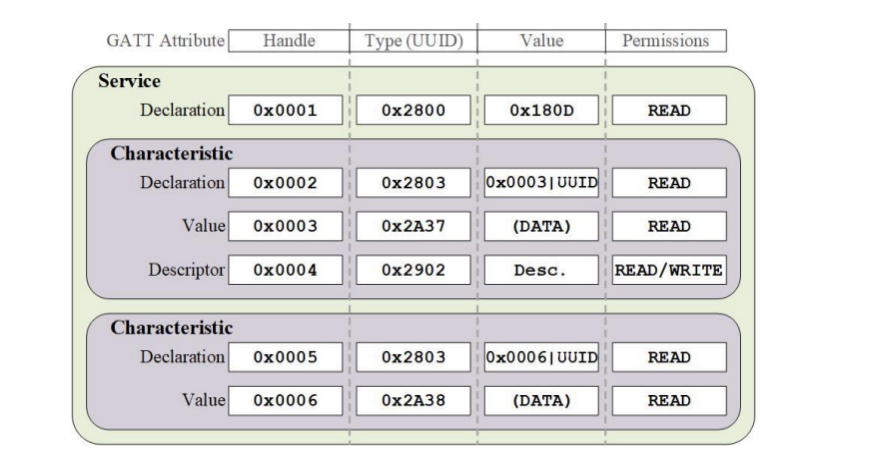
\includegraphics[width=16cm,height=8cm]{Images/System/fmECG_BLE_system.png}
  \caption[Cấu trúc dữ liệu gói]{\bfseries \fontsize{12pt}{0pt}\selectfont Cấu trúc dữ liệu gói}
  \label{fmECG_BLE_system} %đặt tên cho ảnh
\end{figure}
Services được xem như một tập hợp thông tin được thiết kế để đảm bảo thực hiện một chức năng cụ thể. Các Service, chẳng hạn như Battery Service hoặc Sensor Service, được sử dụng để cung cấp các chức năng riêng biệt. Bên trong mỗi Service, một hoặc nhiều Characteristic được định nghĩa để đảm nhận các nhiệm vụ hoặc thông tin cụ thể liên quan đến chức năng của Service đó. UUID (Universal Unique Identifier) được sử dụng để định danh duy nhất toàn cầu cho từng Service và Characteristic.

Dựa trên các cơ sở này, việc lắng nghe và nhận dữ liệu từ thiết bị điện tim cần được thực hiện thông qua kết nối đúng với các Services và Characteristics tương ứng. Trong thiết bị đo điện tim được sử dụng trong đồ án này, các UUID tiêu chuẩn (được biểu diễn dưới dạng chuỗi String) đã được xác định và áp dụng để đảm bảo việc thu nhận dữ liệu từ thiết bị được thực hiện một cách chính xác và hiệu quả:

\begin{adjustwidth}{1.5em}{}
  \begin{itemize}
    \item UUID Service: 6E400001-B5A3-F393-E0A9-E50E24DCCA9E
    \item UUID Characteristic: 6E400003-B5A3-F393-E0A9-E50E24DCCA9E
  \end{itemize}
  \end{adjustwidth}

\begin{figure}[H]
    \centering
    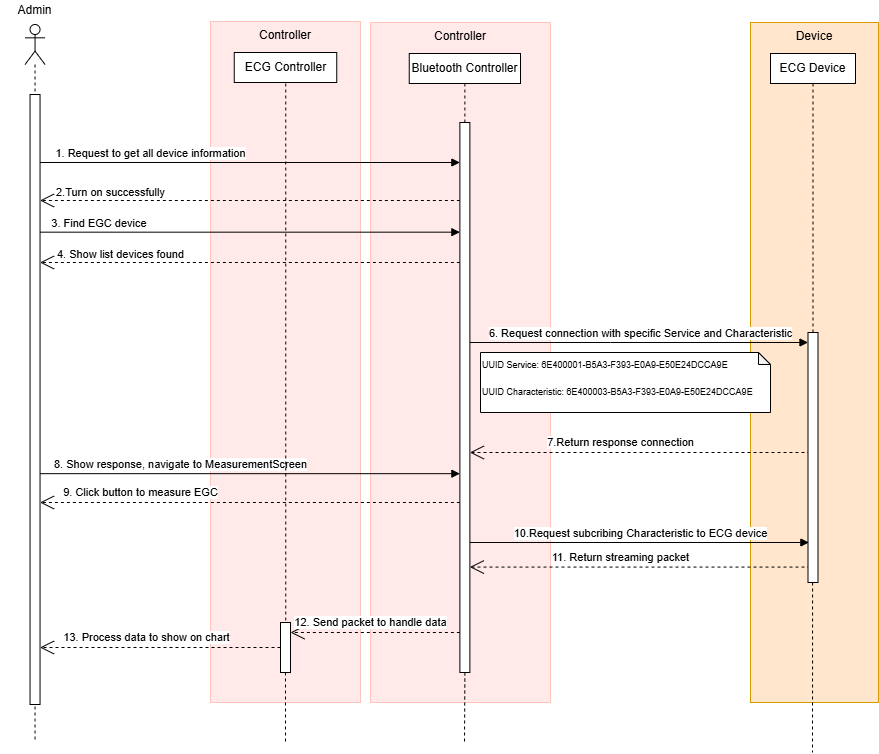
\includegraphics[width=12cm,height=12cm]{Images/System/BLE_system.drawio.png}
    \caption[Sơ đồ tuần tự thiết kế chức năng kết nối và nhận dữ liệu điện tim real-time]{\bfseries \fontsize{12pt}{0pt}\selectfont Sơ đồ tuần tự thiết kế chức năng kết nối và nhận dữ liệu điện tim real-time}
    \label{BLE_system} %đặt tên cho ảnh
  \end{figure}
\subsection{Phân tích dữ liệu}

Tại phần này, chúng em sẽ tiến hành xác định và mô tả các thực thể cũng như
 thuộc tính trong hệ thống. Việc này giúp chúng em có thể nắm được các phần chính 
 trong việc thiết kế nên cơ sở dữ liệu.

Đầu tiên, chúng em sẽ xác định các thực thể và mô tả thuộc tính của nó trong hệ
thống dươi dạng bảng và sơ đồ mô hình liên kết. 


Sau khi hoàn thành được bảng thực thể và thuộc tính, chúng em xác định được mô hình thực thể liên kết như sau:

\subsection{Kết luận}

Chương này thực hiện phân tích khái quát về
 hệ thống, nhằm đáp ứng các yêu cầu và mục tiêu đã được đề ra trong các phần trên.

\newpage
